% Progress-meeting slides — master thesis, Sapienza
% Compile: pdflatex progress_meeting_sandrokh_131026.tex (twice) or latexmk -pdf progress_meeting_sandrokh_131026.tex. Figures: python make_figures.py
% Speaker notes: change "hide notes" to "show notes on second screen=right" to see them.
\documentclass[aspectratio=169,10pt,t]{beamer}

\usepackage[T1]{fontenc}
\usepackage[utf8]{inputenc}
\usepackage{lmodern}
\usepackage{booktabs}
\usepackage{array}
\usepackage{graphicx}
\usepackage{amsmath}
\usepackage{tikz}
\usetikzlibrary{arrows.meta,positioning,calc,fit}
\usepackage{pgfpages}
\setbeameroption{hide notes}          % or: show notes on second screen=right

% ---------- plain theme, minimal colour scheme ----------
\usetheme{default}
\definecolor{ink}{HTML}{1F3A5F}        % dark blue: titles, structure
\definecolor{inkgrey}{HTML}{5A5A5A}
\definecolor{paleline}{HTML}{C8D0DA}
\setbeamercolor{structure}{fg=ink}
\setbeamercolor{frametitle}{fg=ink}
\setbeamercolor{title}{fg=ink}
\setbeamercolor{section in toc}{fg=ink}
\setbeamercolor{alerted text}{fg=ink}
\setbeamercolor{footline}{fg=inkgrey}
\setbeamerfont{frametitle}{size=\large,series=\bfseries}
\setbeamerfont{footline}{size=\scriptsize}
\setbeamertemplate{navigation symbols}{}
\setbeamertemplate{itemize items}{\textcolor{ink}{\textbullet}}
\setbeamertemplate{enumerate items}[default]
\setbeamertemplate{frametitle}{%
  \vspace{0.6em}\insertframetitle\par
  \vspace{0.15em}{\color{paleline}\rule{\textwidth}{0.4pt}}}
\setbeamertemplate{footline}{%
  \hspace{0.8em}\usebeamerfont{footline}\insertshorttitle\ --- \insertshortauthor
  \hfill\insertsection\hfill\insertframenumber\,/\,\inserttotalframenumber\hspace{0.8em}\vspace{0.4em}}
\setlength{\leftmargini}{1.2em}
\setbeamercolor{notebox}{bg=black!8,fg=black}     % grey callout box for one-line messages
% keybox: grey callout with the bullet block centred and bold. Rows of a natural-width tabular,
% so the block sits in the middle of the box; \item starts a new row (one line per bullet).
% Optional argument = font switch for the text (default \bfseries; \mdseries for plain).
\newif\ifkeyboxfirst
\newcommand{\keyboxrow}{\ifkeyboxfirst\global\keyboxfirstfalse\else\\[2pt]\fi\usebeamertemplate{itemize item}~}
\newenvironment{keybox}[1][\bfseries]{\par\smallskip\noindent\global\keyboxfirsttrue
  \let\item\keyboxrow
  \begin{beamercolorbox}[rounded=true,sep=4pt,center,wd=\textwidth]{notebox}
  \begin{tabular}{@{}>{#1}l@{}}}{\end{tabular}\end{beamercolorbox}}

\renewcommand{\cite}[1]{\textcolor{inkgrey}{(#1)}}   % plain (Author et al., year) citations
\usepackage{colortbl}                              % whole-cell shading (slide 16)
\definecolor{greenhi}{HTML}{00441B}   % Greens colormap: highest of the three
\definecolor{greenmid}{HTML}{3A8448}
\definecolor{greenlo}{HTML}{74C476}   % lowest
\newcommand{\shadehi}[1]{\cellcolor{greenhi}\textcolor{white}{#1}}
\newcommand{\shademid}[1]{\cellcolor{greenmid}\textcolor{white}{#1}}
\newcommand{\shadelo}[1]{\cellcolor{greenlo}\textcolor{white}{#1}}
\newcommand{\todo}[1]{\textcolor{red}{[TODO#1]}}
\newcommand{\src}{\mathbf{h}_{\mathrm{src}}}
\newcommand{\dst}{\mathbf{h}_{\mathrm{dst}}}

\title[GNNs for money-laundering detection]{GNN for Fraudulent Pattern Detection}
\subtitle{How do Graph Neural Networks identify money-laundering patterns in a transaction network?\\[0.3em]
          \normalsize Progress meeting\\[0.8em]
          \raisebox{-0.35cm}[1.1cm][0pt]{
\includegraphics[height=1.1cm]{figures/sapienzalogo.pdf}}}
\author[S. Khizanishvili]{Sandro Khizanishvili}
\institute{Supervisor: Prof. Aris Anagnostopoulos\\ Co-supervisor: Loris Cino\\ Sapienza University of Rome}
\date{October 2026}

\begin{document}

% ===================================================================== 1 title
\begin{frame}[plain,c]
  \titlepage
  \note{Thesis in progress: a controlled study of how GNNs detect laundering on a transaction graph.
        Today: what was built, the comparison of four operators over seven feature settings, and
        what is running now. About 15 minutes.}
\end{frame}

% ===================================================================== 2 outline
\begin{frame}[c]{Outline}
  \tableofcontents
  \note{Four parts: the problem, data and the fixed architecture, the results of 28 runs, and the
        two extensions, RWPE node encodings and the data-tuned GFP sheet, with their results.
        Then a short summary and the next steps.}
\end{frame}

% ===================================================================== INTRODUCTION
\section{Introduction}

\begin{frame}{Problem and goal}
  \vspace{1.5em}
  \par\smallskip\noindent
  \begin{beamercolorbox}[rounded=true,sep=4pt,wd=\textwidth]{notebox}\vspace{-0.5em}
    \begin{itemize}
      \item \textbf{Task:} classify each transaction in a transaction graph as laundering or not
      \item \textbf{Question:} can GNNs find laundering patterns, and do graph features help?
    \end{itemize}\vspace{-0.5em}
  \end{beamercolorbox}
  \note{Accounts are nodes, transactions are directed edges, so this is edge classification on a
        temporal multigraph at a 1 : 1,120 imbalance. Laundering shows up as structure (cycles,
        fan-in/out, scatter-gather). Message-passing GNNs are bounded by 1-WL (Xu et al., 2019) and
        cannot count cycles, hence the two routes: a more expressive operator,
        or pre-computed graph features (GFP, Altman et al., 2023).}
\end{frame}

% ===================================================================== DATA & METHOD
\section{Data and Methodology}

\begin{frame}{Dataset}
  \begin{columns}[T]
    \begin{column}{0.52\textwidth}
      \begin{table}
        \small
        \begin{tabular}{@{}ll@{}}
          \toprule
          Property & Value \\
          \midrule
          Source & HI-Small \cite{Altman et al., 2023} \\
          Transactions & 5{,}078{,}345 $\to$ 5{,}077{,}237 \\
          Laundering & 4{,}522 (0.089\,\%) \\
          Accounts (nodes) & 515{,}070 \\
          Time span & 2022-09-01 $\to$ 2022-09-10 \\
          Currencies & 15, converted to USD \\
          Annotated attempts & 370, in 8 typologies \\
          Split by time & 60\,\% train, 20\,\% val, 20\,\% test \\
          \bottomrule
        \end{tabular}
      \end{table}
    \end{column}
    \begin{column}{0.46\textwidth}
      \centering
      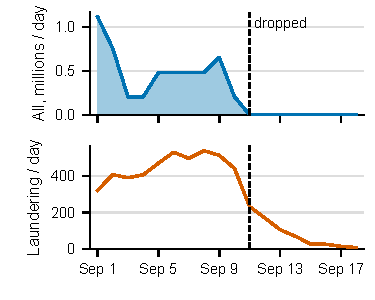
\includegraphics{figures/fig_daily.pdf}
    \end{column}
  \end{columns}
  \vspace{-0.2em}
  \begin{keybox}
    \item Real data ends Sep 10; later days hold only launderers' transactions
  \end{keybox}
  \note{Synthetic but realistic benchmark from IBM with ground-truth labels. The dataset creator
        confirms the days after Sep 10 hold only completions of laundering patterns (the dropped
        tail was 59 \% laundering), which would poison a temporal test split. The eight typologies
        are the ground truth for the per-typology analysis planned later.}
\end{frame}

\begin{frame}{Features}
  \vspace{-0.9em}
  \begin{table}
    \scriptsize
    \setlength{\tabcolsep}{3pt}
    \renewcommand{\arraystretch}{0.92}
    \begin{tabular}{@{}lrl@{}}
      \toprule
      Feature & Dim & What it captures \\
      \midrule
      \multicolumn{3}{@{}l}{\textbf{Node features (6 per account)}} \\
      \addlinespace[1pt]
      \texttt{EntityType\_*} & 6 & kind of account holder (one-hot) \\
      \addlinespace[2pt]
      \midrule
      \multicolumn{3}{@{}l}{\textbf{Baseline edge features (20 per transaction)}} \\
      \addlinespace[1pt]
      \texttt{Amount\_Log} & 1 & amount in USD, log scale \\
      \texttt{Struct\_Band} & 1 & amount just below the \$10k reporting threshold \\
      \texttt{Hour\_Sin/Cos}, \texttt{DayOfWeek\_Sin/Cos} & 4 & time of day and day of week (cyclic) \\
      \texttt{Is\_Weekend} & 1 & weekend flag \\
      \texttt{Is\_Self\_Loop} & 1 & sender and receiver are the same account \\
      \texttt{Same\_Bank} & 1 & sender and receiver at the same bank \\
      \texttt{Dt\_Src\_Log}, \texttt{Dt\_Dst\_Log} & 2 & time since the sender's / receiver's previous transaction \\
      \texttt{Src\_Bank\_Risk}, \texttt{Dst\_Bank\_Risk} & 2 & past laundering rate of the sender's / receiver's bank \\
      \texttt{PayFmt\_*} & 7 & payment channel, one-hot (ACH, Bitcoin, Cash, Cheque, Card, Reinvestment, Wire) \\
      \addlinespace[2pt]
      \midrule
      \multicolumn{3}{@{}l}{\textbf{GFP edge features (61 per transaction)}} \\
      \addlinespace[1pt]
      Scatter--gather & 3 & scatter--gather patterns the transaction belongs to, by size \\
      Temporal cycles & 3 & time-ordered cycles the transaction closes, by length \\
      Simple cycles & 3 & cycles up to length 6 the transaction closes, by length \\
      Vertex statistics & 52 & fan, degree, amount and timing statistics of sender and receiver \\
      \bottomrule
    \end{tabular}
  \end{table}
  \note{GFP is IBM's Graph Feature Preprocessor (Altman et al., 2023) with the paper's windows,
        computed causally in batches of 128. Split: train 3,046,342 edges (2,297 laundering),
        validation 1,015,447 (1,082), test 1,015,448 (1,143); boundaries fixed before feature
        engineering, all fitted quantities use the train window only, test is scored once.}
\end{frame}

\begin{frame}{Fixed architecture}
  \centering
  \resizebox{\textwidth}{!}{%
  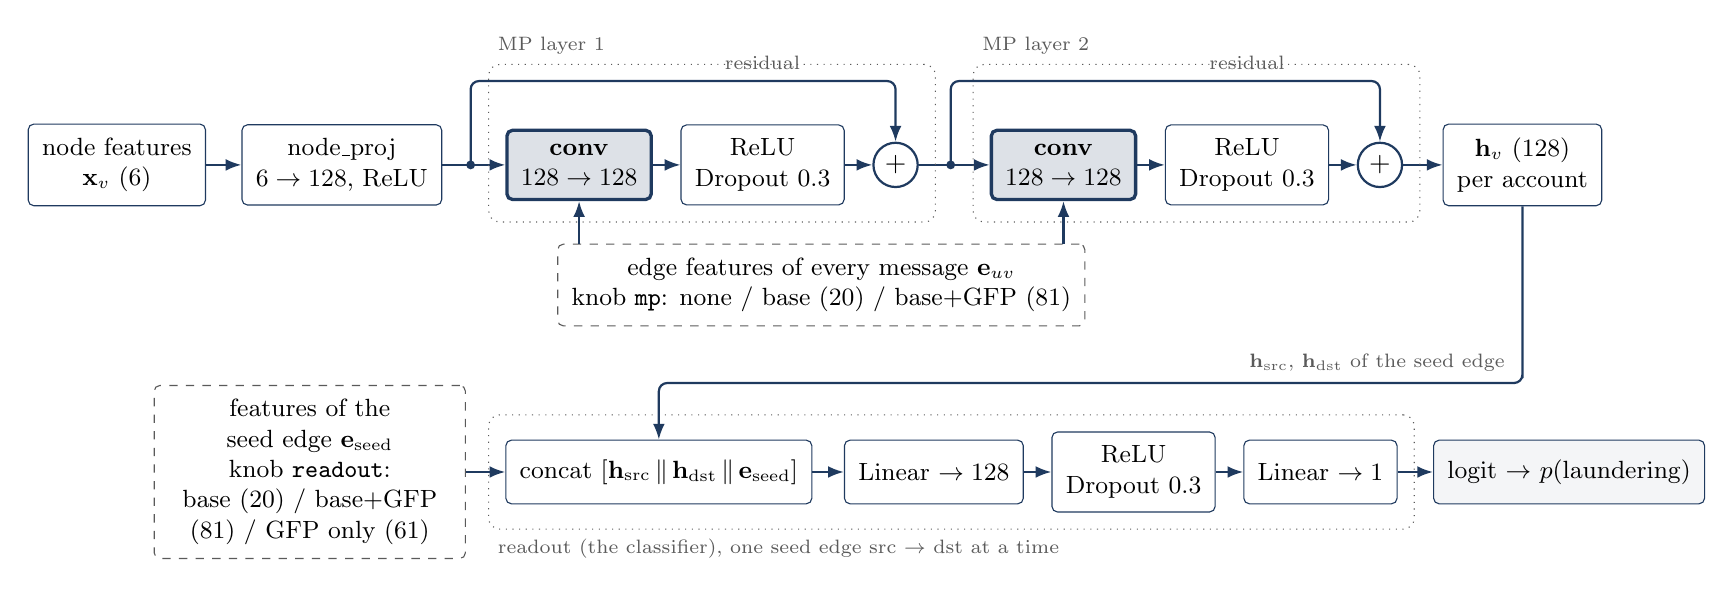
\begin{tikzpicture}[
      font=\small,
      box/.style={draw=ink, rounded corners=2pt, minimum height=2.3em, inner sep=5pt, align=center, fill=white},
      conv/.style={box, fill=ink!15, very thick},
      knob/.style={box, draw=inkgrey, dashed, fill=white},
      sum/.style={draw=ink, circle, thick, inner sep=1pt, minimum size=1.6em, font=\normalsize, fill=white},
      group/.style={draw=inkgrey, rounded corners=4pt, dotted, inner sep=6pt},
      arr/.style={-{Latex[length=2mm]}, ink, thick},
      res/.style={-{Latex[length=2mm]}, ink, thick, rounded corners=3pt},
      lbl/.style={font=\scriptsize, color=inkgrey}]
    % ---- row 1: node path through the two message-passing layers
    \node[box] (x) at (0,0) {node features\\$\mathbf{x}_v$ (6)};
    \node[box, right=0.45cm of x] (proj) {node\_proj\\$6 \to 128$, ReLU};
    \node[conv, right=0.8cm of proj] (c1) {\textbf{conv}\\$128 \to 128$};
    \node[box, right=0.35cm of c1] (a1) {ReLU\\Dropout 0.3};
    \node[sum, right=0.35cm of a1] (s1) {$+$};
    \node[conv, right=0.9cm of s1] (c2) {\textbf{conv}\\$128 \to 128$};
    \node[box, right=0.35cm of c2] (a2) {ReLU\\Dropout 0.3};
    \node[sum, right=0.35cm of a2] (s2) {$+$};
    \node[box, right=0.5cm of s2] (h) {$\mathbf{h}_v$ (128)\\per account};
    \draw[arr] (x) -- (proj);
    \draw[arr] (proj) -- (c1);
    \draw[arr] (c1) -- (a1);
    \draw[arr] (a1) -- (s1);
    \draw[arr] (s1) -- (c2);
    \draw[arr] (c2) -- (a2);
    \draw[arr] (a2) -- (s2);
    \draw[arr] (s2) -- (h);
    % residual skips: branch before the conv, add after the dropout
    \coordinate (r1) at ($(proj.east)!0.45!(c1.west)$);
    \coordinate (r2) at ($(s1.east)!0.45!(c2.west)$);
    \coordinate (top1) at ($(a1.north)+(0,0.55)$);
    \coordinate (top2) at ($(a2.north)+(0,0.55)$);
    \fill[ink] (r1) circle (1.6pt);
    \fill[ink] (r2) circle (1.6pt);
    \draw[res] (r1) |- (top1) -| (s1.north);
    \draw[res] (r2) |- (top2) -| (s2.north);
    \node[lbl, above=0.02cm of top1] {residual};
    \node[lbl, above=0.02cm of top2] {residual};
    % layer groups
    \node[group, fit=(c1)(a1)(s1)(top1)] (g1) {};
    \node[group, fit=(c2)(a2)(s2)(top2)] (g2) {};
    \node[lbl, anchor=south west] at (g1.north west) {MP layer 1};
    \node[lbl, anchor=south west] at (g2.north west) {MP layer 2};
    % ---- edge features entering the convolutions (knob mp)
    \node[knob, below=1.0cm of $(c1)!0.5!(c2)$] (euv) {edge features of every message $\mathbf{e}_{uv}$\\
          knob \texttt{mp}: none / base (20) / base+GFP (81)};
    \draw[arr] (c1 |- euv.north) -- (c1.south);
    \draw[arr] (c2 |- euv.north) -- (c2.south);
    % ---- row 2: readout on the seed edge
    \node[box, anchor=west] (cat) at (c1.west |- 0,-3.9) {concat $[\mathbf{h}_{\mathrm{src}} \,\|\, \mathbf{h}_{\mathrm{dst}} \,\|\, \mathbf{e}_{\mathrm{seed}}]$};
    \node[box, right=0.4cm of cat] (l1) {Linear $\to 128$};
    \node[box, right=0.35cm of l1] (ra) {ReLU\\Dropout 0.3};
    \node[box, right=0.35cm of ra] (l2) {Linear $\to 1$};
    \node[box, right=0.45cm of l2, fill=ink!5] (out) {logit $\to$ $p(\text{laundering})$};
    \draw[arr] (cat) -- (l1);
    \draw[arr] (l1) -- (ra);
    \draw[arr] (ra) -- (l2);
    \draw[arr] (l2) -- (out);
    \node[group, fit=(cat)(l1)(ra)(l2)] (g3) {};
    \node[lbl, anchor=north west] at (g3.south west) {readout (the classifier), one seed edge src $\to$ dst at a time};
    \node[knob, left=0.5cm of cat, text width=3.6cm] (es) {features of the seed edge $\mathbf{e}_{\mathrm{seed}}$\\
          knob \texttt{readout}:\\base (20) / base+GFP (81) / GFP only (61)};
    \draw[arr] (es) -- (cat);
    % node states of the two endpoints feed the readout
    \coordinate (mid) at ($(euv.south)!0.5!(cat.north)$);
    \draw[res] (h.south) |- (h.south |- mid) -| (cat.north);
    \node[lbl, anchor=south east] at ($(h.south |- mid)+(-0.1,0.02)$) {$\mathbf{h}_{\mathrm{src}}$, $\mathbf{h}_{\mathrm{dst}}$ of the seed edge};
  \end{tikzpicture}}

  \vspace{0.4em}
  \begin{keybox}
    \item Only the shaded conv layer changes between runs
  \end{keybox}
  \note{The shaded conv is GIN, GATv2, PNA or the Graph Transformer. Adding features only widens the
        dashed inputs; the training setup is the same for every run. Operators: GIN/GINE (Xu et al., 2019; Hu et al., 2020), GATv2 (Brody et al., 2022), PNA
        (Corso et al., 2020), TransformerConv (Shi et al., 2021); 4 heads x 32 for the two attention
        operators. Hidden 128, 2 layers, dropout 0.3, residual in every layer. Training, identical
        for every run: 100 neighbours per hop, 8,192 seed edges per batch, BCE with pos_weight 8,
        Adam 1e-3 with cosine schedule, 20 epochs, seed 42. The invariant parameter count is the
        same across the seven configurations of a family.}
\end{frame}

\begin{frame}{Seven feature configurations and training setup}
  \begin{table}
    \footnotesize
    \setlength{\tabcolsep}{5pt}
    \begin{tabular}{@{}lccccccc@{}}
      \toprule
      Configuration & 1 & 2 & 3 & 4 & 5 & 6 & 7 \\
      \midrule
      Edge features in MP & none & base & none & base+GFP & base & base & none \\
      Edge features at readout & base & base & base+GFP & base+GFP & base+GFP & GFP only & GFP only \\
      \bottomrule
    \end{tabular}
  \end{table}
  \vspace{-0.3em}
  \begin{table}
    \footnotesize
    \setlength{\tabcolsep}{5pt}
    \renewcommand{\arraystretch}{0.92}
    \begin{tabular}{@{}ll@{}}
      \toprule
      Training setting & Value \\
      \midrule
      Neighbour sampling & 100 per hop, 2 hops \\
      Batch & 8{,}192 seed edges \\
      Loss & BCE, pos\_weight 8 \\
      Optimiser & Adam \\
      Learning rate & $10^{-3}$, cosine schedule \\
      Epochs & 20 \\
      Hidden width & 128 \\
      Message-passing layers & 2 \\
      Dropout & 0.3 \\
      Checkpoint & best validation F1 \\
      Seed & 42 \\
      \bottomrule
    \end{tabular}
  \end{table}
  \note{base = the 20 transaction features, GFP = the 61 graph-pattern features, base+GFP = 81.
        Seven configurations times four operators = 28 runs, all finished. Adam weight decay 1e-5.
        The threshold is swept on validation every epoch; the best-val-F1 checkpoint and its
        threshold are kept and test is scored once with them. Headline metric: minority-class F1. PR-AUC and recall at 5 \% are the secondary metrics; ROC-AUC is
        about 0.97 everywhere and uninformative at this imbalance.}
\end{frame}

% ===================================================================== RESULTS
\section{Results}

\begin{frame}{All configurations per operator}
  \centering
  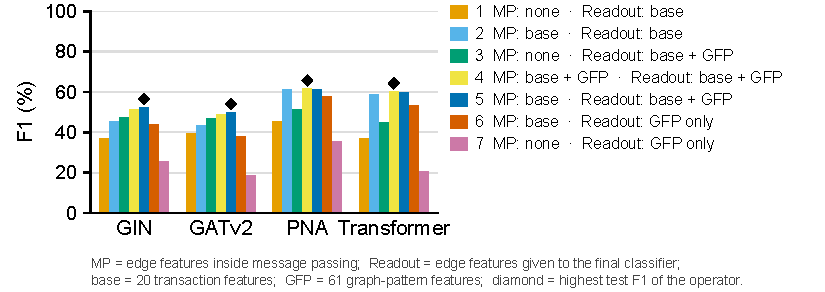
\includegraphics{figures/fig_results.pdf}
  \begin{keybox}
    \item Edge features in message passing help every operator
  \end{keybox}
  \note{Also on the slide: GFP at the readout helps GIN and GATv2, with no clear gain for PNA and the
        Transformer; GFP alone (config 7) is always the worst. Test F1 of all 28 runs, single seed. The 1 to 2 gain is +0.09 for GIN, +0.04 for GATv2,
        +0.16 for PNA and +0.22 for the Transformer: it scales with how the operator uses the edge
        features (GATv2 only reweights attention; PNA and the Transformer add them to the message).
        GFP at the readout (2 to 5) adds +0.07 for GIN and GATv2 and nothing measurable for PNA and
        the Transformer. Diamonds mark the highest test F1 of each operator; the configuration
        chosen by validation F1 (slide 9) is the same for GIN and the Transformer and a tie
        within 0.02 for GATv2 and PNA.}
\end{frame}

\begin{frame}{Test F1 and PR-AUC of all runs}
  \vspace{-0.8em}
  \begin{table}
    \small
    \setlength{\tabcolsep}{2.5pt}
    \renewcommand{\arraystretch}{0.95}
    \begin{tabular}{@{}l*{7}{>{\centering\arraybackslash}p{1.5cm}}@{}}
      \toprule
      Configuration & 1 & 2 & 3 & 4 & 5 & 6 & 7 \\
      \textit{MP} & none & base & none & base+GFP & base & base & none \\
      \textit{Readout} & base & base & base+GFP & base+GFP & base+GFP & GFP only & GFP only \\
      \midrule
      \multicolumn{8}{@{}l}{\textbf{F1 (\%)}} \\
      GIN & \cellcolor[HTML]{5EAB64}\textcolor{white}{37.1} & \cellcolor[HTML]{3E894C}\textcolor{white}{45.6} & \cellcolor[HTML]{367F45}\textcolor{white}{47.1} & \cellcolor[HTML]{28703A}\textcolor{white}{51.2} & \cellcolor[HTML]{246B37}\textcolor{white}{52.5} & \cellcolor[HTML]{4C9856}\textcolor{white}{43.9} & \cellcolor[HTML]{6BBA6F}\textcolor{white}{25.6} \\
      GATv2 & \cellcolor[HTML]{55A25E}\textcolor{white}{39.2} & \cellcolor[HTML]{509D5A}\textcolor{white}{43.5} & \cellcolor[HTML]{3A8448}\textcolor{white}{46.9} & \cellcolor[HTML]{317A42}\textcolor{white}{48.8} & \cellcolor[HTML]{2D753E}\textcolor{white}{50.0} & \cellcolor[HTML]{59A661}\textcolor{white}{37.9} & \cellcolor[HTML]{74C476}\textcolor{white}{18.4} \\
      PNA & \cellcolor[HTML]{438E50}\textcolor{white}{45.2} & \cellcolor[HTML]{04491E}\textcolor{white}{61.4} & \cellcolor[HTML]{28703A}\textcolor{white}{51.2} & \cellcolor[HTML]{00441B}\textcolor{white}{61.7} & \cellcolor[HTML]{094E22}\textcolor{white}{61.1} & \cellcolor[HTML]{1B6230}\textcolor{white}{57.5} & \cellcolor[HTML]{67B56C}\textcolor{white}{35.6} \\
      Transformer & \cellcolor[HTML]{62B068}\textcolor{white}{37.0} & \cellcolor[HTML]{165D2C}\textcolor{white}{58.6} & \cellcolor[HTML]{479353}\textcolor{white}{44.8} & \cellcolor[HTML]{0D5326}\textcolor{white}{60.2} & \cellcolor[HTML]{125829}\textcolor{white}{59.8} & \cellcolor[HTML]{1F6634}\textcolor{white}{53.4} & \cellcolor[HTML]{70BF72}\textcolor{white}{20.4} \\
      \midrule
      \multicolumn{8}{@{}l}{\textbf{PR-AUC (\%)}} \\
      GIN & \cellcolor[HTML]{5DAA64}\textcolor{white}{32.8} & \cellcolor[HTML]{4A9655}\textcolor{white}{39.2} & \cellcolor[HTML]{388147}\textcolor{white}{43.5} & \cellcolor[HTML]{256D38}\textcolor{white}{47.9} & \cellcolor[HTML]{206834}\textcolor{white}{48.4} & \cellcolor[HTML]{469152}\textcolor{white}{39.5} & \cellcolor[HTML]{6BBA6F}\textcolor{white}{19.8} \\
      GATv2 & \cellcolor[HTML]{58A560}\textcolor{white}{33.0} & \cellcolor[HTML]{4F9B59}\textcolor{white}{38.9} & \cellcolor[HTML]{3C874A}\textcolor{white}{41.9} & \cellcolor[HTML]{2E773F}\textcolor{white}{45.8} & \cellcolor[HTML]{337C43}\textcolor{white}{45.1} & \cellcolor[HTML]{61B067}\textcolor{white}{31.2} & \cellcolor[HTML]{74C476}\textcolor{white}{11.2} \\
      PNA & \cellcolor[HTML]{4F9B59}\textcolor{white}{38.9} & \cellcolor[HTML]{00441B}\textcolor{white}{57.8} & \cellcolor[HTML]{2A723C}\textcolor{white}{47.2} & \cellcolor[HTML]{05491F}\textcolor{white}{57.5} & \cellcolor[HTML]{094E22}\textcolor{white}{57.4} & \cellcolor[HTML]{175E2D}\textcolor{white}{54.0} & \cellcolor[HTML]{66B56B}\textcolor{white}{29.0} \\
      Transformer & \cellcolor[HTML]{54A05D}\textcolor{white}{33.7} & \cellcolor[HTML]{13582A}\textcolor{white}{54.9} & \cellcolor[HTML]{418C4E}\textcolor{white}{41.1} & \cellcolor[HTML]{094E22}\textcolor{white}{57.4} & \cellcolor[HTML]{0E5326}\textcolor{white}{55.3} & \cellcolor[HTML]{1C6331}\textcolor{white}{50.8} & \cellcolor[HTML]{6FBF72}\textcolor{white}{13.9} \\
      \bottomrule
    \end{tabular}
  \end{table}
  \vspace{-0.4em}
  \begin{keybox}
    \item PNA and the Transformer lead on both F1 and PR-AUC
  \end{keybox}
  \note{Each model was trained once (one seed); repeated runs are needed for a robust estimate.
        Best of each operator: PNA 61.7 F1 / 57.8 PR-AUC, Transformer 60.2 / 57.4, GIN 52.5 / 48.4,
        GATv2 50.0 / 45.8.
        Test metrics; F1 at the validation-chosen threshold, PR-AUC threshold-free. Green shade follows the rank of the value within each metric (28 runs): lightest = lowest, darkest = highest, evenly spaced steps.
        PNA and the Transformer tie
        at about 0.60 test F1, GIN and GATv2 at about 0.50. PNA has 562k to 623k parameters against
        103k to 132k for GIN and GATv2 and 169k to 197k for the Transformer, so its lead belongs to
        the whole operator. The Transformer uses local attention over the sampled neighbourhood
        only. Test is below validation in every run; no sign of leakage. A seed sweep on the
        winners is planned.}
\end{frame}

\begin{frame}{How our runs compare with the dataset paper (HI-Small)}
  \vspace{-0.4em}
  \begin{table}
    \small
    \setlength{\tabcolsep}{5pt}
    \renewcommand{\arraystretch}{1.05}
    \begin{tabular}{@{}lcccc@{}}
      \toprule
      & \multicolumn{2}{c}{Edge features} & This work & Altman et al. 2023$^{*}$ \\
      \cmidrule(lr){2-3}
      Model & MP & Readout & \textit{F1 (\%), one seed} & \textit{F1 (\%), 4 seeds} \\
      \midrule
      GIN & base & base+GFP & \cellcolor[HTML]{246C37}\textcolor{white}{52.5} & \cellcolor[HTML]{74C476}\textcolor{white}{28.7 $\pm$ 1.1} \\
      GATv2 & base & base+GFP & \cellcolor[HTML]{2C753E}\textcolor{white}{50.0} & NA \\
      PNA & base & base & \cellcolor[HTML]{064B20}\textcolor{white}{61.4} & \cellcolor[HTML]{165C2C}\textcolor{white}{56.8 $\pm$ 2.4} \\
      Transformer & base+GFP & base+GFP & \cellcolor[HTML]{0A4F23}\textcolor{white}{60.2} & NA \\
      GFP + LightGBM & -- & base+GFP & NA & \cellcolor[HTML]{01451C}\textcolor{white}{62.9 $\pm$ 0.3} \\
      GFP + XGBoost & -- & base+GFP & NA & \cellcolor[HTML]{00441B}\textcolor{white}{63.2 $\pm$ 0.2} \\
      \bottomrule
    \end{tabular}
  \end{table}
  \vspace{-0.6em}
  {\scriptsize\color{inkgrey}$^{*}$ The paper's GNNs use 4 base edge features (timestamp, amount received,
   received currency, payment format) in both MP and readout, and a constant node feature of 1s.\par}
  \vspace{0.2em}
  \begin{keybox}
    \item We beat the paper's GIN and PNA, but not its tree models
  \end{keybox}
  \note{Test-set minority-class F1. Paper values from Table 2 of Altman et al. (2023), same 60/20/20
        temporal split and 100/100 neighbour sampling as ours; the paper has no GATv2 or Transformer
        run and we have no tree run yet (planned cross-check). MP and Readout describe our runs
        (GIN config 5, GATv2 config 5, PNA config 2, Transformer config 4); the paper's GNNs are
        base / base, with base = the 4 features in the footnote, projected once and reused at the
        readout. Green shade is the slide-9 scale applied to the value: lightest = 28.7, darkest =
        63.2, linear in between. The paper also reports GIN with edge updates at 47.7 $\pm$ 7.9, a
        step we do not use; our GIN config 2 (base / base) scores 45.6, so the GIN claim holds on
        like-for-like inputs too.
        Caveats: the paper uses the full HI-Small, we removed the laundering-only tail days after
        10 Sep 2022, so our test window is stricter. The paper tuned depth, width (hidden 64),
        learning rate and dropout per model and averages four seeds; we fixed one architecture
        (hidden 128) and ran one seed. Our threshold is chosen on validation; the paper's GNNs use
        the default decision rule (argmax, i.e. 0.5). The paper's GFP counts simple cycles up to
        length 10; our V0 sheet follows its Appendix D except the cycle cap.}
\end{frame}

% ===================================================================== ONGOING
\section{Extensions: RWPE and GFP V1}

\begin{frame}{RWPE node encodings: what and why}
  \begin{table}
    \begin{tabular}{@{}lrrr@{}}
      \toprule
      RWPE & train & val & test \\
      \midrule
      Accounts on a cycle & 0.58\,\% & 1.02\,\% & 1.63\,\% \\
      \bottomrule
    \end{tabular}
  \end{table}
  \vspace{-0.3em}
  \begin{table}
    \begin{tabular}{@{}lr@{}}
      \toprule
      Cycle length to cover & hops \\
      \midrule
      GFP cycle cap (V0) & 6 \\
      GFP cycle cap (paper) & 10 \\
      Longest annotated cycle & 12 \\
      \midrule
      RWPE walk length $k$ & 16 \\
      \bottomrule
    \end{tabular}
  \end{table}
  \begin{keybox}
    \item The random walk follows the direction of the money
    \item Walk length 16 covers the longest cycle, 12 hops
  \end{keybox}
  \note{RWPE = for each account, the probability that a k-step random walk returns to it, steps 1
        to 16, on the directed transaction graph with self-loops dropped, one vector per snapshot.
        Non-zero only for accounts on a directed cycle of length at most k, about 1 \% of accounts.
        k = 16 was chosen a priori (EXPERIMENTS.md appendix) to cover the GFP cycle cap of 6 and
        the paper's 10 with margin; the later measurement of the annotated rings (longest 12) is
        inside that margin. k = 8 was to be tried only if k = 16 showed an uplift. Only the node
        projection widens (+2,048 parameters); invariant parameters unchanged.}
\end{frame}

\begin{frame}{RWPE results: with vs without}
  \centering
  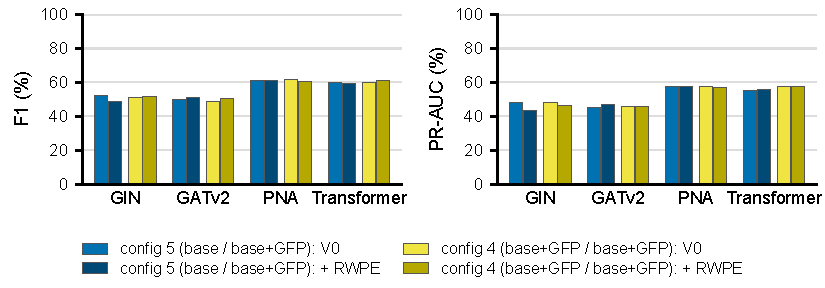
\includegraphics{figures/fig_rwpe.pdf}
  \begin{keybox}
    \item No clear uplift from RWPE on test F1 or PR-AUC
  \end{keybox}
  \note{Decided on validation F1 against the family's own config 5 / 4 run; test shown, never used to
        choose. Validation gaps: GIN -0.011 / -0.004, GATv2 +0.022 / -0.000, PNA +0.001 / -0.004,
        Transformer -0.005 / -0.008. The GATv2 uplift came as higher recall at a lower threshold,
        not better ranking (validation PR-AUC 0.515 vs 0.498). Reading: RWPE is non-zero for under
        2 \% of accounts and GFP at the readout already encodes those cycles. Caveat: on val and
        test the snapshot RWPE also sees edges later than the seed edge, so it is if anything
        optimistic, which makes the null result the safer conclusion. GIN config 5 loses test
        PR-AUC with RWPE (0.484 to 0.435), inside noise on validation but worth a repeat. Batch:
        5.9 h, 21 to 77 min per run.}
\end{frame}

\begin{frame}{GFP V1, tuned to the data: settings}
  \vspace{-0.4em}
  \begin{table}
    \footnotesize
    \setlength{\tabcolsep}{4pt}
    \begin{tabular}{@{}l>{\raggedright\arraybackslash}p{3.8cm}c>{\raggedright\arraybackslash}p{2.6cm}>{\raggedright\arraybackslash}p{2.9cm}@{}}
      \toprule
      GFP feature group & What it counts & \# & V0 & V1 \\
      \midrule
      Scatter--gather & patterns completed, by size & 3 / 4 & 6\,h & 12\,h \\
      \addlinespace[2pt]
      Temporal cycles & time-ordered cycles closed, by length & 3 / 4 & 24\,h & 48\,h \\
      \addlinespace[2pt]
      Simple cycles & cycles closed, any order, by length & 3 / 4 & 24\,h, $\le 6$ hops & 48\,h, $\le 12$ hops \\
      \addlinespace[2pt]
      Pattern bins & size / length bins of the three groups above & -- & [2, 3, 5] $\to$ 3 bins & [2, 4, 6, 8] $\to$ 4 bins \\
      \addlinespace[2pt]
      Vertex statistics & fan, degree, ratio; avg, sum, var, skew, kurt of amounts and times (sender / receiver, in / out) & 52 / 52 & 24\,h & 48\,h \\
      \addlinespace[2pt]
      Graph memory & memory of past transactions & -- & 24\,h & 48\,h \\
      \midrule
      Total per transaction & & 61 / 64 & & \\
      \bottomrule
    \end{tabular}
  \end{table}
  \note{V1 is called `tuned' in the repository, notebooks and docs. Configs 4 and 5 of every operator were
        retrained with V1: 8 runs. Nine of twenty GFP parameters change, one factor group at a time: windows, cycle length,
        bins. The scatter-gather window (12 h) is the one value without measured support: 0 \% of
        scatter-gather attempts fit in 6 h and 2 \% in 12 h, recorded as a known limitation. Graph
        memory must grow with the windows because snapml drops older edges (verified: 48 h cycle
        features with 24 h memory came out identical to 24 h). Before training, the strongest
        label correlation moved from the 2-3-hop cycle bin (+0.064, V0) to the 4-5-hop bin (+0.088,
        tuned); the new 6-7 and 8+ bins stay near zero.}
\end{frame}

\begin{frame}{Why tune GFP: the 370 annotated attempts}
  \vspace{-1.0em}
  \begin{columns}[T]
    \begin{column}{0.58\textwidth}
      \begin{table}
        \small
        \setlength{\tabcolsep}{5pt}
        \renewcommand{\arraystretch}{0.9}
        \begin{tabular}{@{}lrrrr@{}}
          \toprule
          Typology & median & $\le 24$\,h & $\le 48$\,h & $\le 120$\,h \\
          & & \textit{V0} & \textit{V1} & \\
          \midrule
          BIPARTITE      & 24\,h  & 47\,\% & 100\,\% & 100\,\% \\
          CYCLE          & 72\,h  & 9\,\%  & 22\,\%  & 100\,\% \\
          FAN-IN         & 85\,h  & 15\,\% & 22\,\%  & 100\,\% \\
          FAN-OUT        & 77\,h  & 21\,\% & 23\,\%  & 100\,\% \\
          GATHER-SCATTER & 151\,h & 16\,\% & 16\,\%  & 31\,\%  \\
          RANDOM         & 46\,h  & 41\,\% & 51\,\%  & 100\,\% \\
          SCATTER-GATHER & 89\,h  & 2\,\%  & 11\,\%  & 100\,\% \\
          STACK          & 73\,h  & 21\,\% & 33\,\%  & 100\,\% \\
          \midrule
          ALL (370)      & 75\,h  & 21\,\% & 35\,\%  & 91\,\%  \\
          \bottomrule
        \end{tabular}
      \end{table}
    \end{column}
    \begin{column}{0.4\textwidth}
      \begin{table}
        \small
        \setlength{\tabcolsep}{5pt}
        \begin{tabular}{@{}lr@{}}
          \toprule
          Cycle length (54) & \\
          \midrule
          range & 2--12 hops \\
          longer than 6 & 37\,\% \\
          \addlinespace[3pt]
          \toprule
          Fan size (88) & \\
          \midrule
          median & 7.5 \\
          max & 16 \\
          \bottomrule
        \end{tabular}
      \end{table}
      \vspace{-0.4em}
      \begin{beamercolorbox}[rounded=true,sep=4pt,center,wd=\linewidth]{notebox}
        \footnotesize
        \begin{tabular}{@{}>{\bfseries}l@{}}
          \usebeamertemplate{itemize item}~Seen whole: V0 21\,\%, V1 35\,\% \\[2pt]
          \usebeamertemplate{itemize item}~Cycles reach 12 hops; V0 stops at 6
        \end{tabular}
      \end{beamercolorbox}
    \end{column}
  \end{columns}
  \vspace{-0.8em}
  \begin{center}
    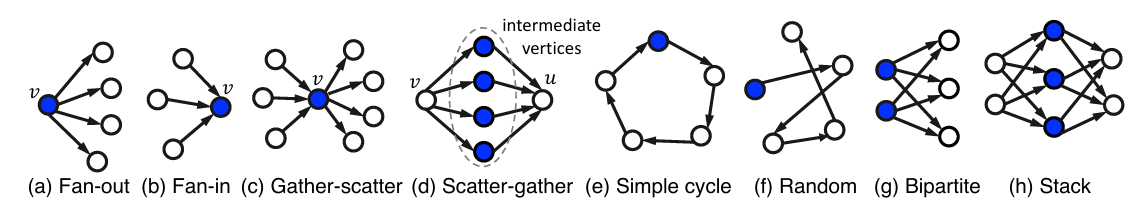
\includegraphics[width=0.68\textwidth]{figures/fig_typologies.png}
  \end{center}
  \note{Typology figure: Altman et al. (2023), Figure 2.
        GFP counts a pattern only when all of its transactions fall inside the window, so the
        percentage columns are the share of attempts GFP can see whole.
        Source: HI-Small\_Patterns.txt (every annotated attempt as a BEGIN/END block with its
        transactions), measured in GFP\_experiments.ipynb section 1. s-g = the scatter-gather
        window (6 h in V0, 12 h in tuned); every other window is 24 h in V0 and 48 h in tuned.
        The paper's windows see a fifth of attempts whole, tuned a third; scatter-gather stays
        almost invisible in both. 120 h would cover nearly everything but was not computed
        (cost, and noise from coincidental long patterns). Not shown: the hop gap, the time a
        middle account waits before passing the money on. In the notebook it is measured for
        cycle and random-walk attempts only (351 hops, median 8.5 h, 96\% within 48 h); for
        stack, scatter-gather and gather-scatter the same measurement gives 71\%, 44\% and 28\%
        within 48 h, so it was dropped from the slide as a one-sided picture.}
\end{frame}

\begin{frame}{GFP results: V0 vs V1}
  \centering
  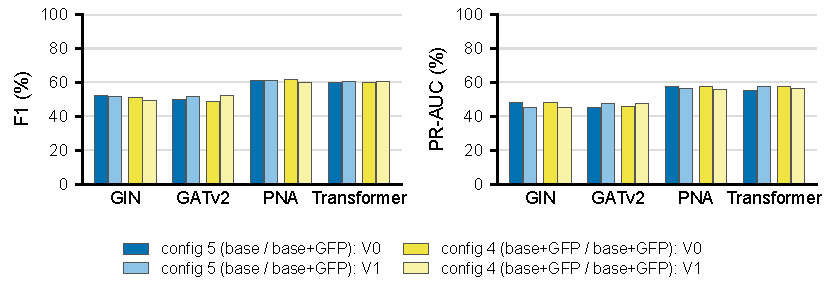
\includegraphics{figures/fig_tuned.pdf}
  \begin{keybox}
    \item Only GATv2 gains from V1; the other operators show no clear gain
  \end{keybox}
  \note{On test: GATv2 gains with V1 in both configs, in F1 and PR-AUC; GIN loses PR-AUC; PNA and
        the Transformer stay inside single-seed noise. V0 stays the default sheet until the GATv2
        gain passes the seed cross-check.
        Validation gaps: GIN -0.004 / -0.004, GATv2 +0.042 / +0.018, PNA +0.005 / -0.003,
        Transformer +0.010 / -0.002. GATv2 is the only operator that moves, on validation and
        test and on both F1 and PR-AUC (config 5: 0.451 to 0.475; config 4: 0.458 to 0.477); it
        is also the operator that profits least from edge features on its own and the only one
        that reacted to RWPE. Whether that is a property of GATv2 or of the weak GAT-5 V0 run
        (still improving at epoch 20) is what the seed cross-check will tell. The tuned sheet
        changes the validation-chosen threshold in every run (PNA-5 0.71 to 0.56, GIN-5 0.50 to
        0.72), trading precision for recall without moving F1. Overfitting unchanged by the
        sheet. Batch: 6.2 h, 23 to 80 min per run.}
\end{frame}

\begin{frame}{All 16 extension runs: test F1 and PR-AUC}
  \begin{table}
    \small
    \setlength{\tabcolsep}{2.5pt}
    \begin{tabular}{@{}ll*{3}{>{\centering\arraybackslash}p{1.6cm}}p{0.3cm}*{3}{>{\centering\arraybackslash}p{1.6cm}}@{}}
      \toprule
      & & \multicolumn{3}{c}{\textbf{F1 (\%)}} & & \multicolumn{3}{c}{\textbf{PR-AUC (\%)}} \\
      \cmidrule(lr){3-5} \cmidrule(lr){7-9}
      Operator & Config & V0 & \makebox[\linewidth][c]{V0 +RWPE} & V1 & & V0 & \makebox[\linewidth][c]{V0 +RWPE} & V1 \\
      \midrule
      GIN & 5 & \shadehi{52.5} & \shadelo{48.6} & \shademid{51.7} & & \shadehi{48.4} & \shadelo{43.5} & \shademid{45.2} \\
      GIN & 4 & \shademid{51.2} & \shadehi{51.9} & \shadelo{49.4} & & \shadehi{47.9} & \shademid{46.5} & \shadelo{45.4} \\
      GATv2 & 5 & \shadelo{50.0} & \shademid{51.3} & \shadehi{51.6} & & \shadelo{45.1} & \shademid{46.9} & \shadehi{47.5} \\
      GATv2 & 4 & \shadelo{48.8} & \shademid{50.2} & \shadehi{52.2} & & \shadelo{45.8} & \shademid{46.0} & \shadehi{47.7} \\
      PNA & 5 & \shademid{61.1} & \shadelo{61.0} & \shadehi{61.3} & & \shademid{57.4} & \shadehi{57.8} & \shadelo{56.5} \\
      PNA & 4 & \shadehi{61.7} & \shademid{60.7} & \shadelo{60.0} & & \shadehi{57.5} & \shademid{56.9} & \shadelo{56.1} \\
      Transformer & 5 & \shademid{59.8} & \shadelo{59.2} & \shadehi{60.7} & & \shadelo{55.3} & \shademid{56.0} & \shadehi{57.4} \\
      Transformer & 4 & \shadelo{60.2} & \shadehi{61.4} & \shademid{60.4} & & \shademid{57.4} & \shadehi{57.5} & \shadelo{56.4} \\
      \bottomrule
    \end{tabular}
  \end{table}
  \begin{keybox}
    \item Only GATv2 improves with both RWPE and V1
  \end{keybox}
  \note{Shading: within each row and metric, darkest = best of the three, lightest = worst. For GATv2
        the order is V1 > V0 +RWPE > V0 in both configs and both metrics; the other operators are mixed.
        V0 = the finished configuration 5 / 4 runs of the main grid (slides 8 and 9); +RWPE adds
        the 16 node features; +tuned swaps the 64-column GFP sheet for V0's 61. Every number is
        test at the validation-chosen threshold, from the batch summaries in Outputs/RWPE and
        Outputs/GFP\_TUNED. Both extensions leave three operators where they were and move only
        GATv2 config 5, by 0.013 to 0.016 F1 on test.}
\end{frame}

% ===================================================================== CONCLUSION
\section{Conclusion}

\begin{frame}{Summary and next steps}
  \textbf{Takeaways}
  \begin{itemize}
    \item One fixed architecture makes all 44 runs comparable
    \item Edge features in message passing lift every operator, most of all PNA and the Transformer
    \item PNA and the Transformer lead; GFP helps only GIN and GATv2
    \item RWPE and GFP V1 improve only GATv2
  \end{itemize}
  \vspace{0.6em}
  \textbf{Next steps}
  \begin{enumerate}
    \item Investigate why GFP V1 does not lift GIN and GATv2 further
    \item Per-typology evaluation of every operator and config
    \item Repeated runs with different seeds for a robust estimate
    \item Global attention: a Transformer over the whole graph, not just local neighbours
    \item Node2Vec node embeddings
    \item GFP V2 with longer time windows
    \item Thesis writing
  \end{enumerate}
  \note{44 runs = 28 of the main grid + 8 RWPE + 8 GFP V1, each trained once with seed 42.
        Per-typology evaluation and the seed sweep come first: they decide whether the GATv2 gains
        and the V1 verdict are real. V0 remains the default GFP sheet until then. The current
        Transformer is local: each layer attends only to direct neighbours (within the sample of 100
        per hop); the global-attention variant lets every node attend to every other node.}
\end{frame}

% ===================================================================== REFERENCES
\section{References}

\begin{frame}{References}
  \scriptsize
  \begin{itemize}
    \item E. Altman, J. Blanu\v{s}a, L. von Niederhäusern, B. Egressy, A. Anghel, K. Atasu.
          \emph{Realistic Synthetic Financial Transactions for Anti-Money Laundering Models.}
          NeurIPS 2023 Datasets and Benchmarks.
    \item K. Xu, W. Hu, J. Leskovec, S. Jegelka. \emph{How Powerful are Graph Neural Networks?} ICLR 2019 (GIN).
    \item W. Hu et al. \emph{Strategies for Pre-training Graph Neural Networks.} ICLR 2020 (GINE edge term).
    \item S. Brody, U. Alon, E. Yahav. \emph{How Attentive are Graph Attention Networks?} ICLR 2022 (GATv2).
    \item G. Corso, L. Cavalleri, D. Beaini, P. Liò, P. Veli\v{c}kovi\'c.
          \emph{Principal Neighbourhood Aggregation for Graph Nets.} NeurIPS 2020 (PNA).
    \item Y. Shi, Z. Huang, S. Feng, H. Zhong, W. Wang, Y. Sun. \emph{Masked Label Prediction: Unified
          Message Passing Model for Semi-Supervised Classification.} IJCAI 2021 (TransformerConv).
    \item V. P. Dwivedi, A. T. Luu, T. Laurent, Y. Bengio, X. Bresson. \emph{Graph Neural Networks with
          Learnable Structural and Positional Representations.} ICLR 2022 (RWPE).
    \item IBM Multi-GNN, reference implementation of the GNN baselines of Altman et al. (2023).
          \texttt{github.com/IBM/Multi-GNN}
    \item IBM Snap ML, \emph{Graph Feature Preprocessor} documentation.
          \texttt{snapml.readthedocs.io/en/latest/graph\_preprocessor.html}
    \item E. Altman. \emph{IBM Transactions for Anti-Money Laundering (AML).} Kaggle dataset and
          discussion \#427517 (laundering-only tail days).
  \end{itemize}
\end{frame}

\end{document}
